\documentclass[tog]{acmsiggraph}

% haha wow, we have so many \thanks{}es that we ran out of symbols to
% use. this is set by the documentclass, so this is sorta breaking the
% rules, but hey, the alternative is to break compilation.
\makeatletter
\let\@fnsymbol\@arabic{}
\makeatother

%%% Used by the ``review'' variation; the online ID will be printed on
%%% every page of the content.
\TOGonlineid{45678}

%%% Used by the ``preprint'' variation.
\TOGvolume{0}
\TOGnumber{0}

\newcommand{\email}[1]{\href{mailto:#1}{\nolinkurl{#1}}}
\newcommand{\emailfoot}[1]{\thanks{\email{#1}}}

\title{S2: STAR Report Introduction, Taxonomy, and Body}

\author{Students: %
 Sanjivi Muttena\emailfoot{sanjivi.muttena@rutgers.edu}, %
 Nikhil Kumar\emailfoot{nikhilkumar516@gmail.com}, %
 Erin Corrado\emailfoot{e.corrado144@gmail.com}, %
 Daniel Bordak\emailfoot{dbordak@fastmail.fm},%
 \\Zooraze Tariq\emailfoot{zooraze@gmail.com}, %
 James Lee\emailfoot{yl50@scarletmail.rutgers.edu}, %
 Krishna Anantha Padmanabhan\emailfoot{krishna.ananth@rutgers.edu}, %
 Jake Taubner\emailfoot{jdt97@scarletmail.rutgers.edu}, %
 Arlind Hoxha\emailfoot{ah621@scarletmail.rutgers.edu}%
 \\Teaching Assistant: Rahul Shome\emailfoot{rahulshome.in@gmail.com}%
 \\Department of Computer Science%
 \\Rutgers University}
\pdfauthor{author1}

\keywords{STAR, S2, Graphics, Introduction, Taxonomy, Body, Machine Learning, Planning, Graph Algorithms, Optimization}

\usepackage{amssymb}
\usepackage{amsmath}
\usepackage{booktabs}
\usepackage{graphicx}
\usepackage{pifont}
\usepackage[usenames, dvipsnames]{color}
\usepackage{tikz}
\usetikzlibrary{graphs, graphs.standard, graphdrawing}
\usegdlibrary{circular}

\graphicspath{ {images/} } %\includegraphics will look for images in the images/ folder

\newcommand{\given}[1][]{\:#1\vert\:}
\newcommand{\reals}{\mathbb{R}}
\newcommand{\cmark}{\color{Green}{\ding{51}}}
\newcommand{\xmark}{\color{Red}{\ding{55}}}
\DeclareMathOperator*{\argmax}{\arg\!\max}

\begin{document}

\maketitle

%\begin{abstract}
%  \paragraph{}
%\end{abstract}

%\begin{CRcatlist}
%  \CRcat{I.3.3}{Computer Graphics}{STAR Topic}{CRcat index}
%  \CRcat{I.3.7}{Computer Graphics}{STAR Topic}{CRcat index};
%\end{CRcatlist}

\keywordlist{}
\setlength{\parskip}{0pt}
\setlength{\parindent}{10pt}

\section{Introduction}

Planning in real time is a challenging task because of the dynamic
nature of environment. A major problem faced by researchers is in
finding an optimal strategy to decide when to expand the state space
and when to stop and recalculate. Another problem faced by researchers
is in expanding algorithms that work with local search to work for
global search where the number of variables increases by a huge
number.

The search domains in real world scenarios are non-deterministic,
complex and huge. This can be owed to the different types of agent’s
viz., characters, objects and obstacles and their behaviors that can
be present in a dynamic environment. Simulating such a domain
virtually is a challenging task due to the large branching factor and
high computational overhead that encompasses it. One of the principal
ways in which we can reduce this overhead is by making use of previous
experiences. This is where machine learning aids, since it
automatically learns, optimizes and plans the agent’s next move based
on previous moves. We need our algorithm to learn the properties of
the search domain and plan accordingly by making use of efficient
heuristic functions and cost functions.

Consider a humanoid robot that can move through any unknown
environment by avoiding all kinds of obstacles, much like C-3PO in
Star Wars. Such a robot would become the state of the art in robotics
and have enormous applications in all aspects of life. These robots
could save lives in the sectors of health, industry, military, etc.
The motion and trajectory planning of this robot would be the most
fundamental, yet formidable challenges of autonomous robotic design.
Since we would have high-dimensional state spaces, using a machine
learning algorithm for its planning stage would be very resource
friendly. The design of such an algorithm is very tricky since we
would have to consider all variables in the robot’s physics but if it
is achieved, we would have a robot that could change our lives
forever.

Machine learning in planning and scheduling can be applied anywhere an
expensive, domain-specific problem exists, and an inexpensive solution
is required; meaning, for businesses that want to make more money, and
academics that need to solve problems with less money. This money is
saved both by reducing required time and optimizing resource use (to
the point it is cost-effective to do so).

Commercial
\begin{itemize}
\item Near-optimal schedules
\item Factory worker scheduling
\item CNC Machine Operation (Lathes, Mills)
\item Production Lines
\item Dispatching
\item Job-shops
\item Analytics
\item Advertising
\item Code repair
\item Data mining
\end{itemize}
Academic
\begin{itemize}
\item Human Learning
\item Mathematical Programming
\item Integer programming problems
\item Empirical Analysis
\item Induction
\item Knowledge-based assistants
\item Geo-coding
\item Data search
\end{itemize}

There are various methods for machine learning and planning because of
its hefty and numerous requirements and features. Each method has its
own purpose and varies depending on the problem to be solved. In order
for machine learning and planning to take place, there needs to exist
a search space, initial and end goal states, and solution. A method
can be evaluated by the following criteria: planning time per move,
likeliness of finding optimal path or near-optimal path, learning
time, and memory usage. Ideally, we want to minimize planning time,
learning time, and memory usage while obtaining as close to optimal
solution as possible. With each of these criteria to keep track of
come with challenges on how to adjust and create a more powerful and
efficient algorithm for machine learning and planning.

The challenges of machine learning and planning is not that of how to
get a solution, but how fast one can get a solution, how efficient the
method is, and how optimal the solution is. There is an abundance of
methods for machine learning and planning, each crafted to solve a
different type of problem. Some methods such as the RTAA* follows
trajectories of smaller cost for given time limits per search because
it updates the heuristics quicker, which allows it to use larger local
search spaces, which overcompensates for its less informed heuristics.~\cite{koenig2006real}
While on the other hand, the min-max LRTA* is expected to run in a
safely explorable state space, meaning the state spaces have to be
relatively small or contain many evenly spread out goal states, but is
inefficient if otherwise.~\cite{koenig1995real} Real-time search does not focus on the
learning aspect but focuses on the time, thus outputting a sub-optimal
solution, but nonetheless a fast solution. Pattern Databases and
Macros can be used to improve performance by making it more efficient
to find states. Hierarchical Task Networks can also be used to help
organize planning algorithms for better efficiency. As one can
observe, there are various trade-offs in efficiency, performance, and
costs, depending on the algorithm's purpose.

As observed in the previous paragraph there are various methods that
are optimal for one scenario but not for another. Since there are a
plethora of problems and solutions under the umbrella of machine
learning and planning, there is no one ``Holy Grail'', but a ``Holy
Grail'' for each problem and solution. We can, however, speculate on
what a ``Holy Grail'' solution would entail. One must observe what is
important in a solution: does the solution need to be obtained as fast
as possible, or does the solution need to be optimal, etc.?
Observation of initial and end goal states along with search space is
also key. If the solution must be optimal and the search space is
small, using the RTAA* would be appropriate since it will output an
optimal solution, but the min-max LRTA* would be preferred over the
RTAA* since the LRTA* is the more optimal in smaller search spaces.~\cite{korf1990real} A
Holy Grail solution would seek to combine the optimality of LRTA* with
the faster speed of RTAA*. Hierarchical Task Networks and Macro
Abstractions are also very useful in making planning algorithms faster
and more efficient. The downside to them is that creating a planning
model from a real-world problem is a difficult and time consuming task
for humans. A long term goal of planning is to create a model that
automatically creates and updates the formulation of a problem.~\cite{botea2005macro}
Therefore, the Holy Grail solution would also include the ability to
automatically and dynamically generate new abstraction models for the
planning, to help with non-deterministic environments.

\section{Prior Work}
The study of machine learning and planning can be broken down into
several categories: Pattern Databases, local search space, Real Time
Adaptive A*, and Learning Real Time A*. Pattern database are
admissible heuristics that are studied and tested on
domain-independent search problems. Another criteria is the use of the
local search space to optimize large scale search problems, while the
use of different planning heuristics is tested and analyzed on
different domains.\cite{haslum2007domain} The primary algorithms of
focus are the Real Time Adaptive A* and Learning Real time A*.
Currently the industry has not fully utilized Machine Learning and AI
for navigation applications. Industry is currently using Incremental
search methods such as dynamic A* for unknown maps. This is used in
DARPA’s Unmanned Ground Vehicle program, Mars Rover, and games such as
Age of Empires 2.

PRODIGY is an architecture used in planning and
learning.\cite{stone1994need} The current frontier of Academic
research is currently focusing on many sections of machine learning
and planning. A study is being done on finding a heuristic method
which can best use machine learning to efficiently handle
domain-independent search problems. Some research is done on reducing
the complexity and the computation need of the algorithm. Another
research method is focused on optimizing this algorithm through aiding
parameters. Research is also being done to help the algorithm solve
larger problems more successfully and expanding its optimal solutions
from the local space into a larger space. Current problems with the
application of machine learning in industry are the difficulty in
extending this problem to multiple monotonous agents. Another problem
is on the balance between exploration and exploitation where most
algorithms have an excessive computation complexity for the optimal
path when good is enough.

\section{Future Work}
Since there exists no ``perfect'' planning algorithm, many open problems
and opportunities for future research exist. One area is pattern
databases; the downfall of pattern databases is that they require a
great deal of memory. Future work to compress pattern databases and
implement them in more efficient and less memory consuming data
structures would be highly useful. RTAA* (Real Time Adaptive A*) could
be extended to work with inconsistent heuristics as well as be
combined with other learning methods such as HTNs. Another area for
future work is using the Macro-FF learning method with complex
structures such as HTNs. Not much research has been done with learning
and HTNs, making this an important area for future research. A long
term open problem is automatic abstraction of planning domains and
problems, as explained in the ``Holy Grail'' solution. Choosing a good
abstraction level for a planning model is a difficult process for a
human, so methods to automatically develop and update the formulation
of a problem is an important area for future work.

\begin{table*}
  \centering
  \begin{tabular}{*{6}{c}}
    \toprule
    & Fast at runtime & Memory Efficient & Real-time & Scalable & Non-deterministic domains \\
    \midrule
    RTAA* & \cmark{} & \cmark{} & \cmark{} & \xmark{}  & \cmark{} \\
    \midrule
    min-max LRTA* & \cmark{} & \cmark{} & \cmark{} & \xmark{}  & \cmark{} \\
    \midrule
    Pattern Databases & \cmark{} & \xmark{} & \xmark{} & \cmark{} & \xmark{} \\
    \midrule
    HTN   & \xmark{} & \cmark{} & \xmark{} & \cmark{} & \xmark{} \\
    \midrule
    Macro Actions & \cmark{} & \cmark{} & \xmark{} & \cmark{} & \xmark{} \\
    \midrule
    Strong AI & \cmark{} & \cmark{} & \cmark{} & \cmark{} & \cmark{} \\
    \bottomrule
  \end{tabular}
  \caption{Feature matrix.}
  \label{table:feature_matrix}
\end{table*}

\section{Overview of Data Structures and Representations}
The entire task of planning in an unknown domain can be broken down
into the following sequence of steps. The first and foremost challenge
is to choose an efficient and space conservative method to store the
data. Since the domains can be large and unknown, the size of the
problem can grow exponentially. This problem escalates even more if
the environment is dynamic. The next challenge is to reach the goal
state from a given state in finite time with the least possible cost.
These solutions will be deployed in real time and it is of utmost
importance that they carry out the action in the given timeframe. If
the environment is not fully observable, then the agents also have to
take into account the probability of change in the portion of the
environment that is not observable. To make planning feasible, we will
take into consideration the data structures and memory
representations.

\subsection{Hierarchical Task Networks}

A Hierarchical Task Network is used to represent dependencies among
actions. The world is represented by a set of states and actions. The
actions represent a transition from one state to another. The reason
why a hierarchical task network is preferred is because it simplifies
the tasks to be performed by decomposing complex tasks into a simple
sequence of primitive actions. To notify the agent on how to decompose
non primitive tasks into subtasks, a set of methods are utilized for
decomposing a particular kind of task into a set of subtasks provided
a set of preconditions are satisfied.~\cite{erol1994htn} For each task, there may be more
than one applicable method, and thus more than one way to decompose
the task into subtasks. For example, in a grid
world representation of a room that has to be cleaned by a vacuum
cleaner agent, a hierarchical task network for the action of cleaning
a room can be decomposed into a set of actions of suck, move right and
move left where the move actions become valid when the grid cell is
clean. One of the task planners that utilize HTNs is the Simple
Hierarchical Ordered Planner (SHOP). A SHOP is domain independent. HTN
planning is in essence a case of decomposition of the entire problem
into subtasks, stopping when it reaches primitive tasks.~\cite{nau1999shop} An ordered
task planner plans in the same way the sequence of actions will be
executed. This reduces the complexity and assumes the deterministic
nature of the environment

\subsection{Pattern Databases}

With the complex actions having been decomposed to a basic set of
primitive tasks, one important data structure that reduces the
complexity exponentially would be pattern databases. A pattern
database holds a collection of solutions to sub problems which have to
be solved to get the overall solution.~\cite{korf2002disjoint} If the amount of space
available is higher, then the solutions to the sub problems can be
precomputed and stored for more efficient and faster calculations.
Essentially, pattern databases work by the comparison of current state
of the decomposed problem to the problem indexed in the database and
returns the precomputed solution.

\subsection{Macro Actions}

To mutate the current state of the environment or agent to the closest
possible recognizable state in the pattern database, a sequence of
actions have to be performed. A macro-action is a meta-action which is
computed from a sequence of action steps. In a planning environment
that involves progressive forward chaining, application of a macro
action to a state produces a successive state that can be obtained by
performing a sequence of actions. In a path finding world, this can be
essentially thought of as an act of extending the path towards the
solution. A good choice leads to an increase in agent performance
while a poor choice raises the branching factor thereby causing the
performance to drop. One of the planners that utilize macros is the
Macro FF planner.~\cite{botea2005macro} An FF planner is a fully automated planner that uses
a heuristic search approach to estimate the best node/state to expand
to reach its goal. The utilization of macros reduces the expansion
factor further since it learns which states to expand and which not
to.

\section{Overview of Search Techniques}

To find out the node that has to be expanded next in the path towards
the goal, the choice has to be made such that the expanded nodes take
us closer to the goal and also compute that optimal solution quickly.
A* search algorithm does give an optimal solution but one major
drawback is the inability to deploy that in very large state spaces
since it would run out of memory before the goal can be reached. Some
variations of A* such as Real Time Adaptive A* and the Learning in
Real Time A* algorithms can be considered viable alternatives
depending on the environments in which the planner has to work on.

\begin{figure}
  \centering
  \begin{tikzpicture}
    % taken from github
    \newcommand{\pacman}[1]{\tikz[baseline=.1em,scale=.6]{
        \useasboundingbox (.02,0) rectangle (.6,.6);
        \draw [fill=#1] (.3,.3) -- ++(25:.3) arc (+25:+335:.3) -- cycle;
    }}

    % taken from github, modified to add mouth
    \newcommand{\ghost}[1]{\tikz[baseline=.1em,scale=.5]{
        \draw [fill=#1] (0,0) -- (0,.5) arc (+180:0:.3) -- (.6,0) --
        (.5,.15) -- (.4,0) -- (.3,.15) -- (.2,0) -- (.1,.15) -- cycle;
        \coordinate (eye) at (360*rand:.03);
        \foreach \x in {.17,.43}{
          \fill[white] (\x,.5) circle[radius=.1];
          %\fill[black] (\x,.5) ++(eye) circle[radius=.05];
        }
        \draw[white](.1,.2) -- (.2,.3) -- (.3,.2) -- (.4,.3) -- (.5,.2);
    }}

    \graph[simple necklace layout]{
      1 -- 2 -- 3 -- 4 -- 5 -- 6 -- 7 -- 8 -- 1;
    };

    \begin{scope}[yshift=-2.5cm]
    \node (1) {
      \tikz \ghost{black!30};
    };
    \end{scope}
    \node (1) {
      \tikz \pacman{white};
    };
  \end{tikzpicture}
  \caption{Hunter/Prey graph. The Hungry Circle seeks to eat the Scared Ghost.}
  \label{fig:hungrycircle}
\end{figure}

A simple example of a nondeterministic graph is that of a hunter
chasing its prey. In this case, the hunter is the agent, and the prey
is its goal. However, the goal can move about randomly. In figure
\ref{fig:hungrycircle}, a Hungry Circle chases a Scared Ghost. So long
as the Ghost continually moves away from the Circle, the goal will
never be met, meaning a search of this graph may take infinite time.

\subsection{Real Time Adaptive A*}

The basic idea behind Real Time Adaptive A* is simple. In an
environment with multiple agents, each agent has to perform A*
repeatedly with the same goal state but with possibly different start
states. But each time A* is performed, the heuristics give a better
estimate so that future A* searches are quicker.~\cite{koenig2006real} A* in general works
by using \(f(s)\) which is the sum of the cost function \(g(s)\) from
start node to current node and heuristic estimate \(h(s)\) from the
current node to the goal state. A priority queue maintains a list of
open nodes and from these set of nodes, the one with the least
\(f(s)\) is chosen for expansion. To make future A* searches faster,
let us consider how the heuristic can be updated. Let \(s\) be a state
expanded during the search process. Obtaining an admissible estimate
for \(gd[s]\) is easy. The distance from the start state
\(s_\text{current}\) to any goal state via state \(s\) is equal to the
sum of distance from the start state \(s_\text{current}\) to state
\(s\) and the goal distance \(gd[s]\) of state \(s\). This is larger
than the goal distance of \(s_\text{current}\). If \(s'\) is the goal
state, then goal distance \(gd[s]\) of state \(s\) is larger than the
goal distance \(gd[scurrent]\) minus the distance from the start state
\(s_\text{current}\) to state \(s\).

\[ g[s] + gd[s] \geq gd[scurr] \]
\[ gd[s] \geq gd[scurr] - g[s] \]
\[ gd[s] \geq f[s'] - g[s] \]

Eventually, the heuristic proposed in this technique is
\[ h[s] = f[s'] - g[s] = g[s'] + h[s'] - g[s] \]

RTAA* doesn’t work when heuristics are inconsistent.

\subsection{Learning Real Time A*}

LRTA* updates the heuristics in a very basic way. For a given state
\(s\), LRTA* with a lookahead of one considers immediate neighbors. We
choose to advance toward the neighbor with the lowest value for
\(f()\), and consider \(s'\) to be the state of this neighbor. If
\(f(s') + 1\) is greater than the current \(f(s)\), then \(f(s)\) is
set to \(f(s') + 1\). Finally, \(s\) is advanced to \(s'\). As far as
LTRA* is concerned, the factors that have to be taken into
consideration are deeper lookaheads, heuristic weights and adding
backtracking so that the heuristics of predecessor nodes can also be
updated.

For non-deterministic domains, min-max LRTA*\cite{koenig2006real} is
proposed. Here, when deciding which neighbor to advance toward, we
consider only the maximum possible value of \(f()\) for each --- in
other words, we always assume a worst-case scenario. In a
deterministic case, there is only one possible value for each, so this
collapses back into regular LRTA*. This min-of-maxes is used again
when setting \(f(s)\), again only when it's value \(+1\) exceeds the
current \(f(s)\).

\section[Modeling a Planning Problem] {Modeling a Planning Problem \footnotemark}
\footnotetext{Throughout this section, the book \textit{Introduction to Stochastic Processes} 
by Erhan \c{C}inlar was referenced  extensively, as were the lectures on artificial intelligence 
from Geoffrey J. Gordon of CMU and Sarah Finney of Harvard.}

%NOTE(jake): the command \c{C} gives you the character Ç

Many planning and reinforcement learning problems occur in partially 
observable stochastic environments. Given a complete model of the 
environment, the problem can be reformulated as a Partially Observable 
Markov Decision Process (POMDP), a technique borrowed from operations 
research. POMDPs generalize Markov Decision Processes (MDPs) to allow 
for the agent to learn. MDPs themselves are an extension of Markov chains, 
allowing the agent to possess a utility function. Many important 
properties of Markov chains and MDPs carry over to POMDPs, so they will 
be briefly discussed first.

\subsection{Markov Chains}

Given a countable state space $S$ and a probability measure $P$ on some 
sample space, a stochastic process $X = \left\{ X_n \given n \in \mathbb{N} \right\}$ 
is said to be a Markov chain if
\begin{equation*}
  P \left( X_{n+1} = s \given X_0, X_1, \ldots, X_n \right) = P \left( X_{n+1} = s \given X_n \right)
\end{equation*}
for all $s \in S$. In other words, at any point in time the process is 
in a well-defined state and the probability that it will transition into 
a different state is dependent only on the current state and not the path 
it took to arrive there. A stochastic process for which this is true is said 
to satisfy the Markov property, or that it simply is Markovian.

\begin{figure}[h]
  \centering
  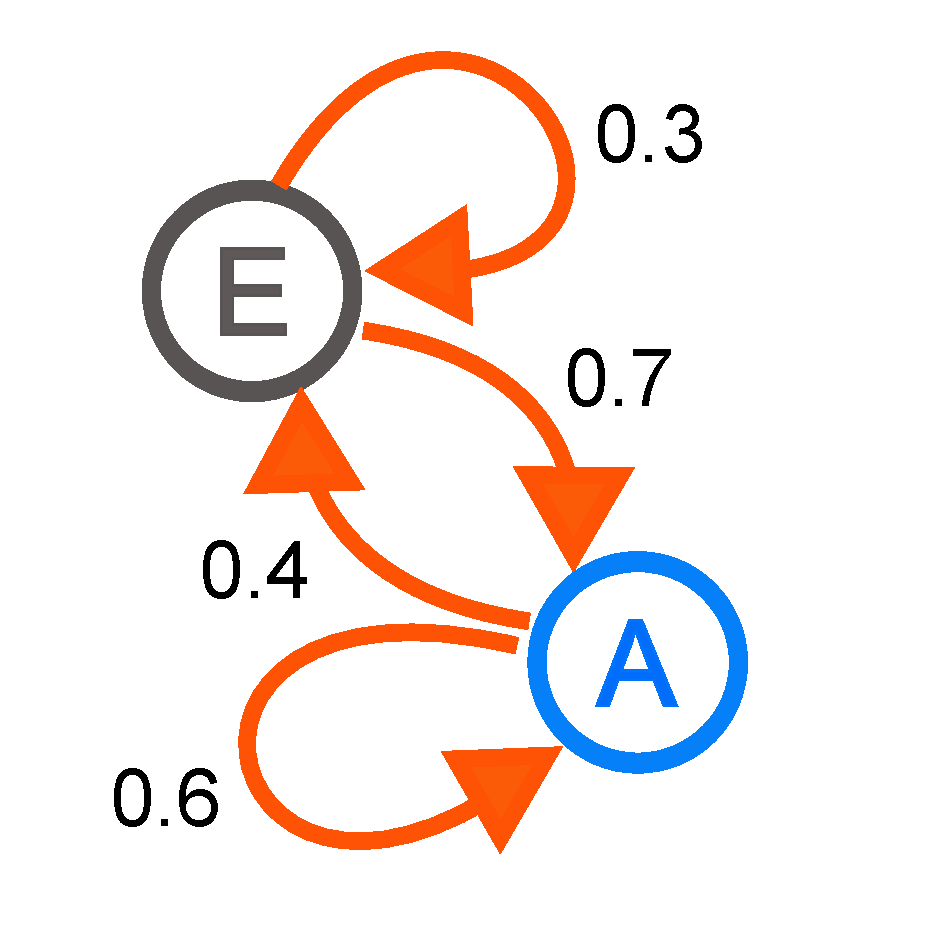
\includegraphics[scale=0.3]{MarkovChain.pdf}
  \caption{A simple two state Markov chain. (Source: Wikipedia)}
  \label{fig:markovChain}
\end{figure}

It is helpful to imagine a Markov chain as a weighted, directed graph $G = (V, E)$, 
in which each vertex $v \in V$ corresponds to a state $s \in S$, and the weight of 
each edge $\left(v, u \right) \in E$ corresponds to the probability of transitioning 
from state $v$ into state $u$, $P \left( X_{n+1} = u \given X_n = v \right)$.

The definition of a Markov chain can be extended to the continuous time case to form 
what is called a Markov process. Given a state space $S$, a time 
$t \in \reals^+ = \left[ 0, \infty \right)$, and a stochastic process 
$X = \left\{ X_t \given t \in \reals^+ \right\}$, we say that $X$ is a 
Markov process if for any $s \in S$, $\epsilon \geq 0$, and all times $\tau \leq t$
\begin{equation*}
  P \left( X_{t+\epsilon} = s \given X_{\tau \leq t} \right) = P \left( X_{t+\epsilon} = s \given X_t \right)
\end{equation*}
The interpretation of this definition is the same as the case of the discrete time Markov chain.

\subsection{Markov Decision Processes}

Ordinary Markov chains are rarely used in planning problems due to their 
limited flexibility. MDPs are a class of discrete time stochastic control 
processes that extend the theory of Markov chains to model Markovian agents 
who have partial control over their environment. Given a countable set of 
states $S$, a countable set of actions $A$, a probability measure 
$P : S \times S \times A \mapsto \left[0, 1 \right]$, a reward function 
$R : S \times A \mapsto \reals$, and a discount factor $\gamma \in \left[0, 1 \right]$,
an MDP $X$ is defined as the 5-tuple
\begin{equation*}
  X = \left(S, A, P, R, \gamma \right)
\end{equation*}

The probability measure for an MDP is sometimes referred to as a transition
 model. For $s, s^\prime \in S $ and $a \in A$, the number $P \left(s, s^\prime , a \right)$
 is the probability that the agent will transition into state $s^\prime$ 
if it takes the action $a$ while in state $s$. $R \left( s, a \right)$ is 
the reward (utility) that the agent will receive if it takes action $a$ while 
in state $s$. The discount factor represents how much the agent discounts 
future rewards. If $\gamma \approx 1$ then rewards in the far future will 
only be discounted slightly relative to the near future, and conversely if 
$\gamma \approx 0$ then rewards in the far future will be heavily discounted.

Let $R_t \in R$ denote the reward an agent receives at time $t$. As usual, 
we are considering the discrete time case $t = 0, 1, \ldots$ so the agent's 
total reward including the discount factor will be
\begin{equation*}
  \sum_{t=0}^\infty \gamma^t R_t
\end{equation*}
Since $\gamma \in \left[0, 1 \right]$, this series will always converge given 
finite valued rewards.

If $A$ and $S$ are finite rather than countably infinite, then an MDP can be solved with 
linear programming or a variety of dynamic programming algorithms. If they are countably 
infinite, then in some cases it is still possible to get an approximate answer by only 
considering a finite subset of the state and action spaces.

\begin{figure}[h]
  \centering
  \def\svgwidth{\columnwidth}
  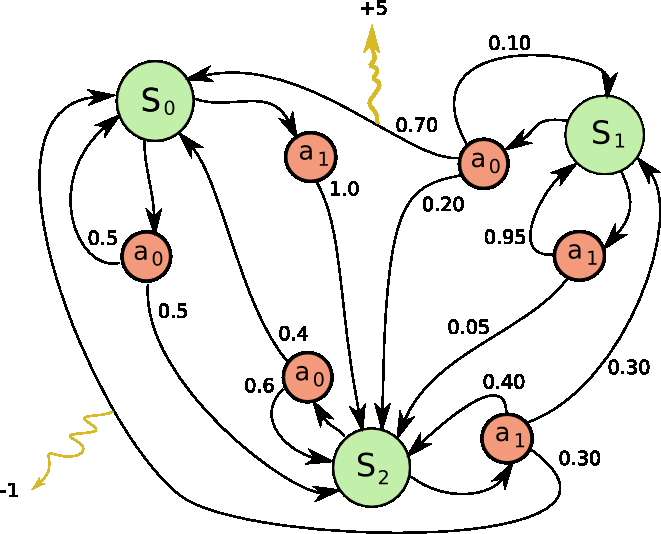
\includegraphics[width=\columnwidth]{MDP.png}
  \caption{A three state MDP with two actions. (Source: Wikipedia)}
  \label{fig:markovDecisionProcess}
\end{figure}

Like Markov chains, it is helpful to imagine MDPs as graphs. However, in this case the vertices 
are not just the states but also actions. The edges of the graph connect states to actions 
and actions to states. There is never an edge which connects an action to another action nor 
a state to another state.

\subsubsection{Policies}
\label{sec:policies}

We have not yet specified how an agent decides which action to take. A policy 
$\pi : S \mapsto A$ is a function which determines what action an agent will take 
at each state. We say than a policy is an optimal policy if it leads to the highest expected utility.

Let $U \left( s_i, a \right) : S \times A \mapsto \reals$ denote the \textit{expected} 
discounted utility of taking action $a$ in state $s_i$. A useful but unenlightening 
way to define an optimal policy is
\begin{equation*}
  \pi \left(s_i \right) = \argmax_{a \in A} U \left( s_i, a \right)
\end{equation*}
This reads almost literally as ``given state $s_i$, choose the action which maximizes 
the expected utility.'' We define $J \left( s_i, a \right)$ as the utility $R_{ia}$ for 
taking action $a$ in state $s_i$ plus the expected discounted utility for taking that 
action. Let $P_{ija}$ denote the probability of transitioning from state $s_i$ into $s_j$ 
after taking action $a$, then
\begin{equation} \label{eqn:U}
  U \left( s_i, a \right) = R_{ia} + \gamma \sum_{j=1}^{\left| S \right|} P_{ija} U \left( s_j, \pi \left( s_j \right) \right)
\end{equation}
Equation~\ref{eqn:U} has the form of a \textit{Bellman Equation}, a famous class of equations in dynamic programming.
We say that $U \left( s_i, a \right)$ satisfies the Bellman equation if
\begin{equation*}
  U \left( s_i, a \right) = \max_{a \in A} R_{ia} + \gamma \sum_{j=1}^{\left| S \right|} P_{ija} U \left( s_j, \pi \left( s_j \right) \right)
\end{equation*}

\begin{figure}[h]
  \centering
  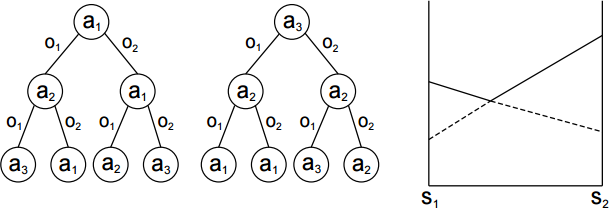
\includegraphics[scale=0.4]{valueTrees.png}
  \caption{Two policies represented as trees and their corresponding utility functions for a two state POMDP.~\protect\cite{hansen2004dynamic}}
  \label{fig:valueTrees}
\end{figure}

\subsection{Solving an MDP}
It is much easier to explain how to solve a POMDP if we first know how to solve an MDP.\@
The solution of an MDP returns an optimal policy, the exact sequence of actions to take 
at each point in time to maximize the agent's utility. For any given MDP, there exists a 
unique optimal policy.

\subsubsection{Value Iteration}

To solve Equation~\ref{eqn:U}, it is convenient to break up the problem by the number 
of steps left and then apply a dynamic programming algorithm known as value iteration. 
Let $U_k \left( s_i, a \right)$ denote the expected utility of taking action $a$ 
in state $s_i$ when there are $k$ steps left in the process, and similarly let 
$\pi_k \left(s_i \right)$ denote the optimal policy for state $s_i$ when there are $k$ steps 
left in the process. Then our definitions from Section~\ref{sec:policies} become
\begin{equation*}
  \begin{split}
    \pi_k \left(s_i \right) &= \argmax_{a \in A} U_k \left( s_i, a \right) \\
    U_k \left( s_i, a \right) &= R_{ia} + \gamma \sum_{j=1}^{\left| S \right|} P_{ija} U_{k-1} \left( s_j, \pi \left( s_j \right) \right)
  \end{split}
\end{equation*}
We also define a base case for when $k=0$,
\begin{equation*}
  U_0 \left( s, a \right) = 0 \quad \forall \left( s, a \right) \in S \times A
\end{equation*}

If there were only a finite amount of steps $K$, then we could iterate over $k = 0, 1, \ldots, K$ 
(as well as $i = 0, 1, \ldots |S|$ and all $a \in A$) and compute each $\pi_k$ and $U_k$. 
However, there is nothing preventing the number of steps from becoming infinite. 
In this case, we choose some $\epsilon > 0$ and stop iterating over $k$ when
\begin{equation*}
  \left| U_k\left( s_i, a \right) - U_{k-1}\left( s_i, a \right) \right| < \epsilon
\end{equation*}
Since $U_k$ is convergent, this condition is guaranteed to occur eventually.

\subsubsection{Policy Iteration}
\label{sec:policyIteration}

Value iteration works by improving our planning policy despite having inaccurate 
estimates of $U_k$. Policy iteration takes the opposite approach and begins with 
any arbitrary policy (or even a completely random one) and obtains accurate estimates 
of $U_k$ before improving the policy. Policy iteration involves two steps: computing 
the utilities $U_k \left(s_i, \pi_k \left(s_i \right) \right)$ for a fixed arbitrary policy, and then 
using the knowledge of these utilities to compute a better policy.

Given some fixed policy $\pi_k$, we compute the utilities much in the same way as before:
\begin{equation*}
    U_k \left( s_i, \pi_k \left( s_j \right) \right) = R_{ia} + \gamma \sum_{j=1}^{\left| S \right|} P_{ija} U_{k-1} \left( s_j, \pi_k \left( s_j \right) \right)
\end{equation*}
and \textit{then} a better policy is calculated,
\begin{equation*}
  \begin{split}
    \pi_k \left(s_i \right) &= \argmax_{a \in A} U_k \left( s_i, a \right) \\
    &= \argmax_{a \in A}  R_{ia} + \gamma \sum_{j=1}^{\left| S \right|} P_{ija} U_{k-1} \left( s_j, a \right)
  \end{split}
\end{equation*}

This method is not guaranteed to return the optimal policy. A different method exists 
where $n$ equations with $n$ unknowns are formed and solved just by using Gauss-Jordan 
elimination. The Gauss-Jordan method has a time complexity of $\mathcal{O} \left( n^3 \right)$, 
where as the previous method is only $\mathcal{O} \left( n^2 \right)$. The Gauss-Jordan 
method, however, is guaranteed to return the optimal policy.

In general, value iteration runs much faster than policy iteration. Policy iteration 
can converge quite fast if a near-optimal policy is known in advance.

\subsection{Partially Observable Markov Decision Processes}

MDPs are useful for modeling environments where the outcome is partially stochastic 
and partially controlled by the decision maker. However, they assume that the agent 
has complete knowledge of the environment \textit{ex-ante}. Because of this, ordinary 
MDPs have no place in reinforcement learning problems and only limited use for planning 
problems. POMDPs are a more generalized version of MDPs which allow the agent to learn 
as it interacts with its environment. This is done by adding two more objects to the tuple: 
a set of possible observations $\Omega$, and a probability measure $O$ corresponding to the 
probabilities of each observation being made given a certain action in a certain state, 
$O = O \left( \omega \in \Omega, s \in S, a \in A \right)$. Thus a POMDP $X$ is defined 
by the 7-tuple
\begin{equation*}
  X = \left(S, A, P, R, \Omega, O, \gamma \right)
\end{equation*}

A ``belief set'' $B$ is typically also part of a POMDP problem. The beliefs $b \left( s \right) \in B$ 
represent a probability distribution over the states $s \in S$. At each time step, 
the agent takes an action $a \in A$ which causes three things happen: the agent transitions 
into a new state $s^\prime \in S$ (like in a Markov chain), the agent receives a utility equal to 
$R \left( s^\prime, a \right)$ (like in an MDP), %TODO(jake): should it be R(s,a)?
and the agent receives an observation $\omega \in \Omega$ about the environment with probability 
$O \left( \omega \given s^\prime, a \right)$ which it then uses to update its beliefs.

The last step is what gives POMDPs their flexibility. Since there are no restrictions on what method 
the agent uses to update its beliefs (other than, of course, that the beliefs should obey the axioms 
of probability), we are free to choose whatever statistical model or machine learning method that's 
appropriate for our system.

Let $\tau$ denote the belief update function. Since POMDPs are Markovian, $\tau$ depends on the 
agent's current beliefs and not beliefs which were previously held. The agent receives a new set 
of beliefs $B^\prime$ by
\begin{equation} \label{eqn:beliefUpdate}
  B^\prime = \tau \left( B, a, \omega \right)
\end{equation}

\begin{figure}[h]
  \centering
  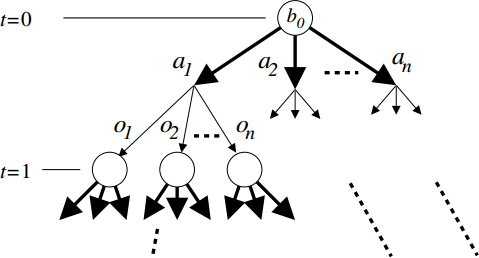
\includegraphics[scale=0.4]{POMDPtree.png}
  \caption{A POMDP represented as a tree.~\protect\cite{smith2004heuristic}}
  \label{fig:POMDPtree}
\end{figure}

\subsubsection{Belief MDP}

These Markovian belief states can be used to reformulate a POMDP as an MDP in which every state 
corresponds to a belief. This new MDP is often referred to as a \textit{belief MDP}. Similar to 
an ordinary MDP, a belief MDP $X$ is defined as a five tuple,

\begin{equation*}
  X = \left(B, A, \tau, r, \gamma \right)
\end{equation*}

where $B$ is the set of belief states, $A$ is the same set of actions from the original POMDP, 
$\tau$ is the belief transition function from Equation~\ref{eqn:beliefUpdate}, and $\gamma$ is 
the same discount factor from the original POMDP. \@ $r$ is a new reward function 
$r: B \times A \mapsto \reals$ which must be derived from the original POMDP.

\subsection{Solving a POMDP}

The exact solution to a POMDP yields the exact sequence of actions that an agent should take 
to maximize the sum of its utilities. The definition of a POMDP allows for countably infinite 
state and action spaces. However, most algorithms for solving POMDPs must assume that the 
state and action spaces are finite. POMDPs can be solved using almost the same methods as MDPs.

\subsubsection{Value Iteration}
While value iteration worked quite well for MDPs, it is much less useful for POMDPs. The use of 
observation probabilities gives POMDPs great modeling power, however it also adds significant 
computational complexity. Performing value iteration on a POMDP is equivalent to performing value 
iteration on a very large number of MDPs, since every belief state represents an MDP on its own. 
Value iteration on POMDPs has a time complexity which is exponential in \textit{both} the number 
of states $|S|$ and the number of actions $|A|$.

\begin{figure}[h]
  \centering
  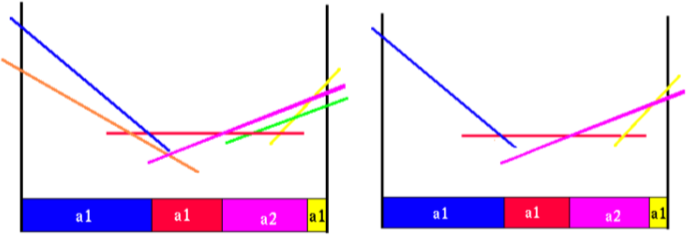
\includegraphics[width=\columnwidth]{combinedValueFunctions.png}
  \caption{Utiltiy functions for taking actions $a_1$ and $a_2$. Dominated vectors are ``pruned'' away. (Source: Geoffrey J. Gordon)}
  \label{fig:combinedValue}
\end{figure}

\subsubsection{Witness Algorithm}
The witness algorithm attempts to improve value iteration by looking for regions where the utility function is suboptimal. Starting with utility vectors which are already known, the witness algorithm runs a linear program based on the Bellman equation which finds a point in the belief space at which the utility function is incorrect. It then calculates a new utility by forming a linear combination of the old utility vectors and adds it to it's working space. This process is iterated as much as is necessary.
\begin{figure}[h]
  \centering
  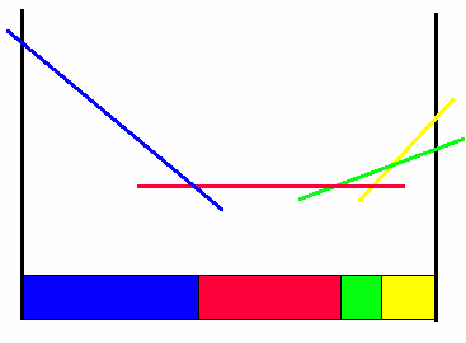
\includegraphics[scale=0.3]{currentValueEstimate.png}
  \caption{Estimate of the utility function during value iteration (Source: Geoffrey J. Gordon)}
  \label{fig:current}
\end{figure}

\begin{figure}[h]
  \centering
  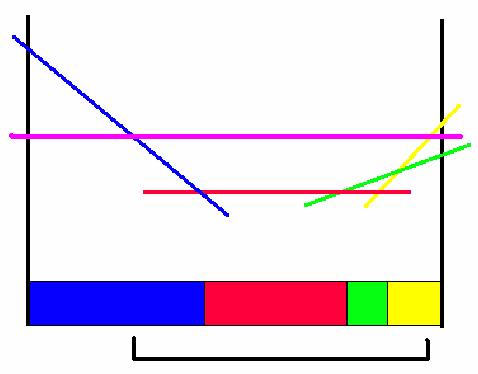
\includegraphics[scale=0.3]{suboptimalWitness.png}
  \caption{The addition of a new vector dominates some of the old vectors. (Source: Geoffrey J. Gordon)}
  \label{fig:current}
\end{figure}

\subsubsection{Policy Iteration}
Although most of what was covered in previous sections was ``textbook'' material, POMDPs remain 
an active area of research to this day. The size of a real-world POMDP problem is large enough 
that it is impossible to solve in a reasonable amount of time. Applying the algorithm described 
in Section~\ref{sec:policyIteration} is highly inefficient. Fortunately, there have been many 
great strides towards improving policy iteration in recent years.

\subsection{Current research in solving POMDPs}

\begin{figure}[h]
  \centering
  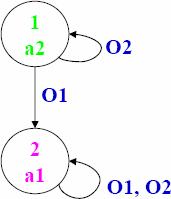
\includegraphics[scale=0.5]{state_controller.png}
  \caption{A simple policy graph. (Source: Geoffrey J. Gordon)}
  \label{fig:state_controller}
\end{figure}
\subsubsection{Policies as Finite-State Controllers}
The inefficiency of policy iteration on POMDPs comes mainly from evaluating the utility 
function for each policy. Efficiency can be greatly improved if the policy is represented 
as a finite-state controller, which we call a \textit{policy graph}.~\cite{hansen1998solving} 
Each vertex represents a vector in the utility function, and each edge represents a state 
transition based on observations.

This gives rise to a new algorithm. As before, given whatever the current policy is, the 
utility function should be calculated. The system of linear equations that the utility function 
represents should be solved, and then the utility function should be updated using the Bellman 
equation. The policy is then updated, and new controllers added if necessary.

\subsubsection{Point-Based Value Iteration}
The main idea behind the Point-Based Value Iteration algorithm is to solve the POMDP for a finite 
set of belief points.~\cite{pineau2003point} New belief points are added to the set when improvements 
after each iterative step are not great enough. The POMDP is solved considering only this finite 
set. A point-based value update takes only polynomial time.

\subsubsection{Heuristic Search Value Iteration}
Heuristic Search Value Iteration (HSVI) is an algorithm which obtains approximate solutions to POMDPs, 
but runs quite fast and scales well to large problems. The main idea behind HSVI is to combine search 
heuristics with a piecewise linear convex representation of the utility function.~\cite{smith2004heuristic} 
The search heuristics greatly reduce the search space by only focusing on the ``most important'' beliefs.

\subsubsection{Continuous State-Action Spaces}
It is possible to solve a POMDP with uncountably infinite state and action spaces by applying Monte Carlo methods. Obviously, since discrete, finite POMDPs are nearly impossible to solve exactly, infinite POMDPs generally can't be solved exactly either. An approximation algorithm (devised by Thrun) known as the MC-POMDP algorithm uses Monte Carlo sampling to represent beliefs and propagate them through time.~\cite{thrun1999monte} As before, a belief state $B_t$ is a Markovian probability distribution over states obtained as a time $t$ conditioned on previous observations $\omega$ and actions $a$,
\begin{equation*}
  B_{t+1} = P \left( X_{t+1} = s_i \given X_t  \right)
\end{equation*}
Let $\alpha \in \reals$ represent a normalization constant (ie a number which normalizes a probability distribution), define $O \left( \omega \given s \right)$ to be the probability of making observation $\omega$ in state $s$. In the MC-POMDP algorithm, belief states are calculated by
\begin{equation*}
  B_{t+1} = \alpha O \left( \omega_{t+1} \given s_{t+1} \right) \int P \left( X_{t+1} = s_{t+1} \given a_t, X_t  \right) ds_t
\end{equation*}

\bibliographystyle{acmsiggraph}
\nocite{*}
\bibliography{S2bibliography.bib}

\end{document}
